\documentclass[12pt,letterpaper]{report}

\usepackage{geometry}
\usepackage{graphicx}

\pagestyle{empty}

% A4     dimensions: 8.268 in x 11.693 in
% Letter dimensions: 8.5   in x 11     in
\geometry{
  body={6.5in, 9.0in},
  left=1.0in,
  top=1.0in
}

\begin{document}

\section*{SensEye Imager/ADC\\Chip-on-Board Mounting and Wirebonding Information}
\begin{figure*}[h!]
 \centering
 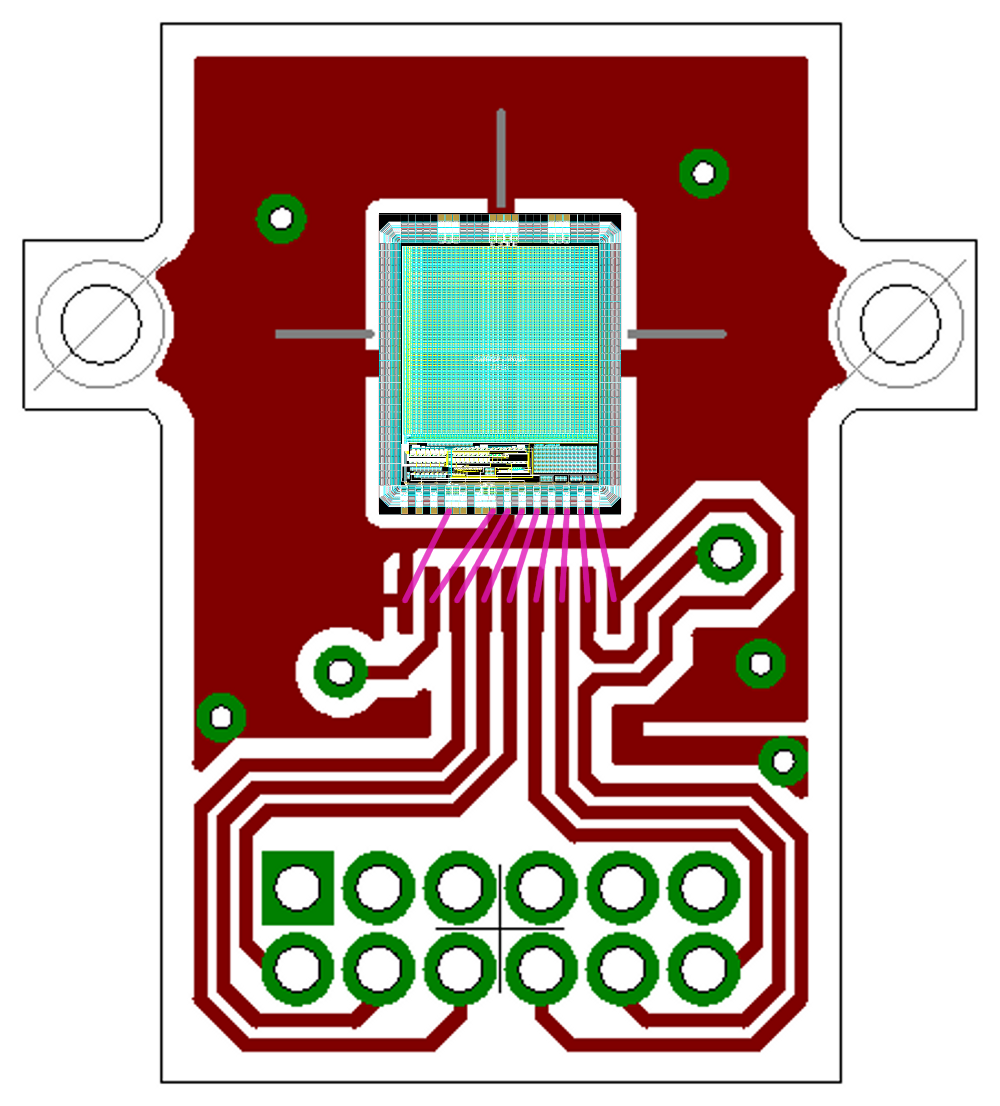
\includegraphics[width=0.92\textwidth]{senseye-imager-adc-wirebonding-diagram.png}
 \caption[b]{\textbf{SensEye Imager/ADC board wirebonding diagram.}}
 \label{fig-wirebonding}
\end{figure*}

\noindent
Figure \ref{fig-wirebonding} shows an image of the top layer of the two-layer
SensEye Imager/ADC PCB with an image of the CentEye Stonyman die superimposed.
This image indicates the orientation of the die on the board, as well as where
the wirebonds are necessary to attach the die pads to the PCB board pads.  The
pad beneath the die is connected to GND, and conductive die attach is preferred,
but not absolutely required.\\

\begin{figure*}[h!]
 \centering
 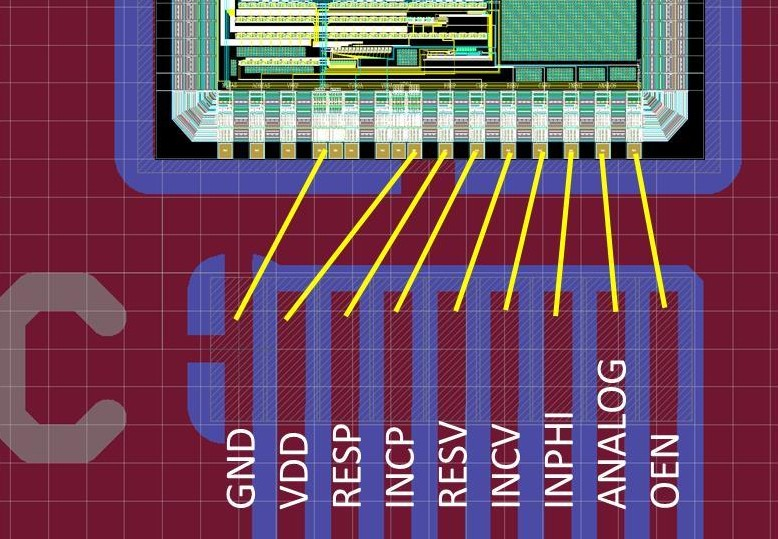
\includegraphics[width=1.0\textwidth]{centeye/stonyman-wirebonding-closeup.jpg}
 \caption[b]{\textbf{Closeup wirebonding diagram.}}
 \label{fig-wirebonding-closeup}
\end{figure*}

\noindent
Figure \ref{fig-wirebonding-closeup} shows a closeup image of the wirebonding
connects required to connect the Stonyman die pads to the PCB board pads.  Nine
wirebonds are required, as labelled: GND, VDD, RESP, INCP, RESV, INCV, INPHI,
ANALOG and OEN.

\begin{table}[h]
   \centering
   \begin{tabular}{|l|l|}
      \hline
      \textbf{Board pad pitch} & 0.016 inch \\
      \hline
      \textbf{Board pad width} & 0.008 inch \\
      \hline
      \textbf{Board pad height} & 0.039 inch \\
      \hline
   \end{tabular}
   \caption{\textbf{PCB board wirebonding pad attributes table.}}
   \label{table-pads-board}
\end{table}

\begin{table}[h]
   \centering
   \begin{tabular}{|l|l|}
      \hline
      \textbf{Die pad pitch (without spacers)} & 0.016 inch \\
      \hline
      \textbf{Die pad pitch (with spacers)} & 0.016 inch \\
      \hline
      \textbf{Die pad width} & 0.008 inch \\
      \hline
      \textbf{Die pad height} & 0.039 inch \\
      \hline
   \end{tabular}
   \caption{\textbf{Stonyman die pad attributes table.}}
   \label{table-pads-die}
\end{table}
\end{document}
